\documentclass[12pt, leqno]{article} %% use to set typesize
\input{common}

\usepackage{fontspec}
\usepackage{polyglossia}
\setmonofont{DejaVu Sans Mono}[Scale=MatchLowercase]
\usepackage[outputdir=pdf]{minted}

\providecommand{\tightlist}{%
  \setlength{\itemsep}{0pt}\setlength{\parskip}{0pt}}
\begin{document}



\hdr{2023-04-12}

\section{Life beyond fixed points}

So far, the methods we have discussed for solving nonlinear systems all
involve some flavor of fixed point iteration \[x^{k+1} = G(x^k).\] Our
chief example of such an iteration is Newton's method, where
\[G(x) = x - f'(x)^{-1} f(x).\] but we have also considered various
other iterations where the Jacobian is replaced by some more convenient
approximation. However, all the methods we have discussed in this
setting compute the next point based only on the behavior at the current
point, and not any previous points.

In earlier parts of the class, of course, we did consider iterations
where the next approximation depends on more than just the current
approximation. Two such iterations spring particularly to mind:

\begin{itemize}
\tightlist
\item
  The secant method is the 1D iteration in which we approximate the
  derivative at the current point by a finite difference through the
  last two points.
\item
  In iterative methods for solving linear systems, we started with fixed
  point iterations based on matrix splittings (such as Jacobi and
  Gauss-Seidel), but then recommended them primarily as an approach to
  preconditioning the more powerful Krylov subspace methods. One way to
  think about (preconditioned) Krylov subspaces is that they are spanned
  by the iterates of one of these stationary methods. Taking a general
  element of this space --- a linear combination of the iterates of the
  stationary method --- improves the convergence of stationary methods.
\end{itemize}

In this lecture, we describe nonlinear analogues to both of these
approaches. The generalization of the secant condition to more than one
direction gives Broyden's method, the most popular of the quasi-Newton
methods that couple a Newton-like update of the approximate solution
with an update for an approximate Jacobian. The generalization of the
Krylov subspace approach leads us to extrapolation methods, and we will
describe a particular example known as reduced rank extrapolation. We
conclude the lecture with a brief discussion of Anderson acceleration, a
method that can be seen as a generalization either of the secant
approach or of Krylov subspace methods.

As with last time, we will continue to use the autocatalytic
reaction-diffusion equation as a running example.

\section{Broyden}

Quasi-Newton methods take the form \[x^{k+1} = x^k - J_k^{-1} f(x^k)\]
together with an updating formula for computing successive approximate
Jacobians \(J_k\). By far the most popular such updating formula is
Broyden's (good) update:
\[J_{k+1} = J_k + \frac{f(x^{k+1}) s^k}{\|s^k\|^2}, \quad s^k = x^{k+1}-x^k\]
Broyden's update satisfies the secant condition
\[J_{k+1} (x^{k+1}-x^k) = f(x^{k+1})-f(x^k)\] which is the natural
generalization of the 1D secant condition. In one dimension, the secant
condition is enough to uniquely determine the Jacobian approximation,
but this is not the case in more than one dimension. Hence, Broyden's
update gives the matrix \(J_{k+1}\) that minimizes \(\|J_{k+1}-J_k\|_F\)
subject to the secant condition.

\begin{minted}{julia}
function naive_broyden(x, f, J; rtol=1e-6, nsteps=100,
                       monitor=(x, fx) -> nothing)

    x = copy(x)
    J = Array{Float64}(J)  # Dense matrix representation of the initial Jacobian

    # Take an initial step to get things started
    fx = f(x)
    monitor(x, fx)
    s = -J\fx
    
    for step = 1:nsteps

        # Take Broyden step and update Jacobian (overwrite old arrays)
        x[:] += s
        fx[:] = f(x)
        J[:,:] += fx*(s/norm(s)^2)'
        s[:] = -J\fx

        # Monitor progress and check for convergence
        monitor(x, fx)
        if norm(fx) < rtol
            return x, fx
        end

    end
    
    # We could error out here, but let's just return x and fx
    return x, fx
end
\end{minted}

Broyden's method has three particularly appealing features:

\begin{itemize}
\tightlist
\item
  For sufficiently good starting points \(x^0\) (and sufficiently
  innocuous initial Jacobian approximations), Broyden's method is
  \(q\)-superlinearly convergent, i.e.~there is some constant \(K\) and
  some \(\alpha > 1\) such that \(\|e^{k+1}\| \leq \|e^k\|^\alpha\).
\item
  The iteration requires only function values. There is no need for
  analytical derivatives.
\item
  Because each step is a rank one update, we can use linear algebra
  tricks to avoid the cost of a full factorization at each step that
  would normally be required for a Newton-type iteration.
\end{itemize}

The argument that Broyden converges superlinearly is somewhat complex,
and we will not cover it in this course; for details of the argument, I
suggest Tim Kelley's
\href{https://doi.org/10.1137/1.9781611970944}{Iterative Methods for
Linear and Nonlinear Equations}. The fact that the method requires only
function values is obvious from the form of the updates. But the linear
algebra tricks bear some further investigation, in part because
different tricks are used depending on the type of problem involved.

\begin{figure}
\begin{center}
  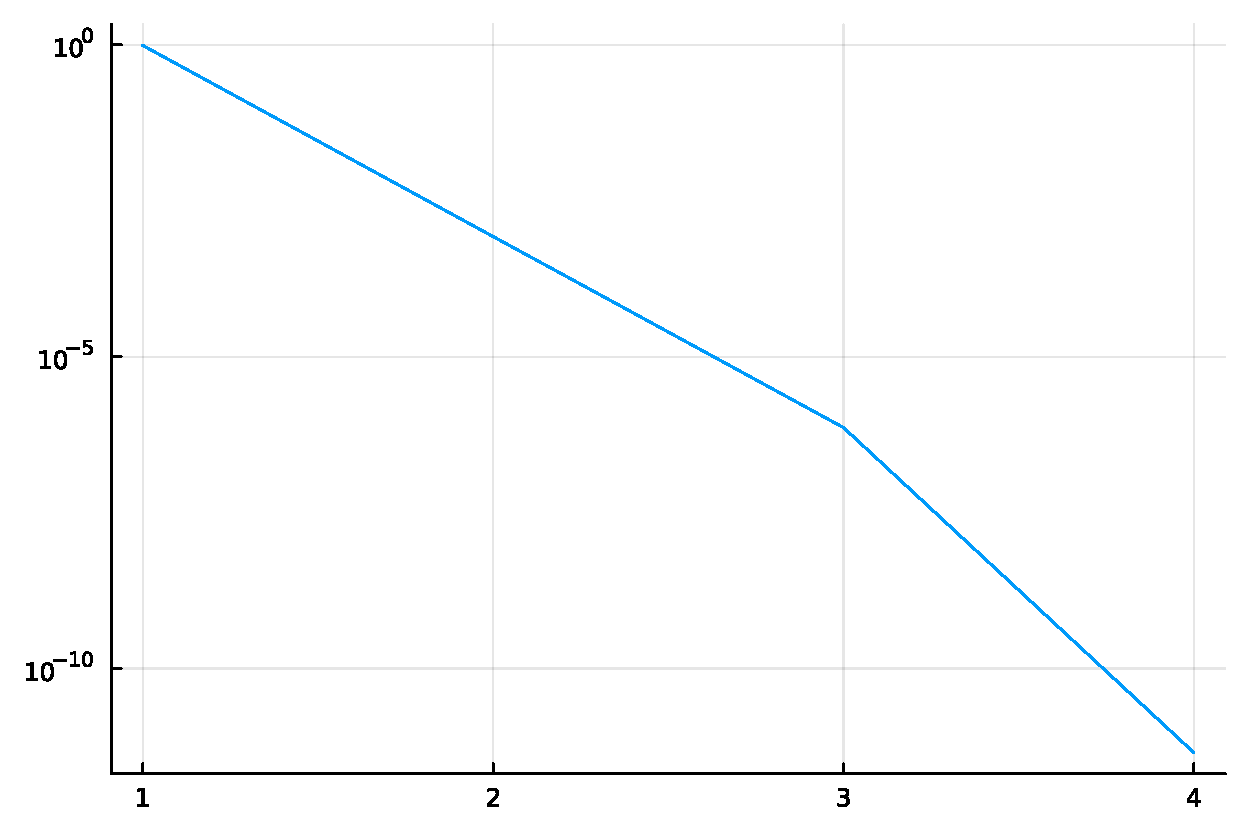
\includegraphics[width=0.8\textwidth]{fig/2023-04-14-broyden-cvg.pdf}
\end{center}
\caption{Convergence of Broyden.}
\label{fig:broyden-cvg}
\end{figure}

We plot convergence of Broyden on the autocatalytic example in
Figure~\ref{fig:broyden-cvg}.  We use the exact Jacobian at the
starting point as our initial Jacobian estimate.

\subsection{Questions}

Give an argument for the claim above that Broyden's update gives the
matrix \(J_{k+1}\) that minimizes \(\|J_{k+1}-J_k\|_F^2\) subject to the
secant condition.

\section{Dense Broyden}

For moderate-sized problems, implementations of Broyden's method may
maintain a dense factorization of the approximate Jacobian which is
updated at each step. This updating can be done economically by
exploiting the fact that the update at each step is rank one. For
example, the QR factorization of \(J_k\) can be updated to a QR
factorization of \(J_{k+1}\) in \(O(n^2)\) time by using a sequence of
Givens rotations. More generally, we can compute the QR factorization of
the rank one update \(A' = A+uv^T\) from the QR factorization
\(A = \bar{Q} \bar{R}\) in three steps:

\begin{enumerate}
\def\labelenumi{\arabic{enumi}.}
\tightlist
\item
  Write \(A' = \bar{Q} (\bar{R} + \bar{u} v^T)\) where
  \(\bar{u} = \bar{Q}^T u\)
\item
  Apply \(n-1\) Givens rotations to \(\bar{u}\) to introduce zeros in
  positions \(n, n-1, \ldots, 2\). Apply those same rotations to the
  corresponding rows of \(R\), transformint it into an upper Hessenberg
  matrix \(H\); and apply the transposed rotations to the corresponding
  columns of \(\bar{Q}\) to get \(A' = \tilde{Q} (H + \gamma e_1 v^T)\).
\item
  Do Hessenberg QR on \(H + \gamma e_1v^T\) to finish the decomposition,
  i.e.~apply Givens rotations to zero out each subdiagonal in turn.
\end{enumerate}

In total, this computation involves computing \(\bar{u}\) (in \(O(n^2)\)
time) and applying \(2n-2\) Givens rotations across the two factors
(also a total of \(O(n^2\) time). So updating the factorization of
\(J_k\) to get a factorization of \(J_{k+1}\) takes \(O(n^2)\); and once
we have a factorization of \(J_{k+1}\), linear solves can be computed in
\(O(n^2)\) time as well. So the total cost per Broyden step is
\(O(n^2)\) (after an initial \(O(n^3)\) factorization).

\begin{minted}{julia}
function qrupdate!(Q, R, u, v)
    n = length(u)
    ubar = Q'*u
    for j = n:-1:2
        G, r = givens(ubar[j-1], ubar[j], j-1, j)
        ubar[j] = 0.
        ubar[j-1] = r
        R[:,j-1:end] = G*R[:,j-1:end]
        Q[:,:] = Q[:,:]*G'
    end
    R[1,:] += ubar[1]*v
    for j = 1:n-1
        G, r = givens(R[j,j], R[j+1,j], j, j+1)
        R[j,j] = r
        R[j+1,j]= 0.
        R[:,j+1:n] = G*R[:,j+1:n]
        Q[:,:] = Q[:,:]*G'
    end
end
\end{minted}

\subsection{Questions}

Complete the following code for Broyden with QR updating.

\begin{minted}{julia}
function dense_broyden(x, f, J; rtol=1e-6, nsteps=100,
                       monitor=(x, fx) -> nothing)

    x = copy(x)            # Copy x (overwrite w/o clobbering the initial guess)
    J = Array{Float64}(J)  # Dense representation of the initial Jacobian
    F = qr(J)              # Get a QR factorization
    Q = Matrix(F.Q)        # Convert the Q factor to standard dense form
    R = F.R                # Extract the R factor
    
    # Take an initial step to get things started
    fx = f(x)
    monitor(x, fx, J)
    s = -J\fx
    
    for step = 1:nsteps
        
        # Take Broyden step and update Jacobian (overwrite old arrays)
        x[:] += s
        fx[:] = f(x)
        
        # TODO: Replace these lines with QR-based version
        J[:,:] += fx*(s/norm(s)^2)'
        s[:] = -J\fx
        
        # Monitor progress and check for convergence
        monitor(x, fx)
        if norm(fx) < rtol
            return x, fx
        end
        
    end
    
    # We could error out here, but let's just return x and fx
    return x, fx
end
\end{minted}

\section{Large-scale Broyden}

For large-scale problems, the \(O(n^2)\) time and storage cost of a
dense Broyden update may be prohibitive, and we would like an
alternative with lower complexity. As long as we have a fast solver for
the initial Jacobian \(J_0\), we can compute the first several Broyden
steps using a bordered linear system
\[\begin{bmatrix} J_0 & -F_k \\ S_K^T & D_k \end{bmatrix}
  \begin{bmatrix} s^k \\ \mu \end{bmatrix} = 
  \begin{bmatrix} -f(x^k) \\ 0 \end{bmatrix},\] where \begin{align*}
  F_k &= \begin{bmatrix} f(x^1) & \ldots & f(x^k) \end{bmatrix}, \\
  S_k &= \begin{bmatrix} s^0 & \ldots s^{k-1} \end{bmatrix}, \\
  D_k &= \operatorname{diag}( \|s^0\|^2, \ldots, \|s^{k-1}\|^2).
\end{align*} Defining vectors \(g^k = -J_0^{-1} f(x^k)\) (chord steps),
we can rewrite the system as
\[\begin{bmatrix} I & G_k \\ S_k^T & D_k \end{bmatrix} 
  \begin{bmatrix} s^k \\ \mu \end{bmatrix} =
  \begin{bmatrix} g^k \\ 0 \end{bmatrix}.\] Defining \(w = -\mu\) and
performing block Gaussian elimination then yields \begin{align*}
  (D_k - S_k^T G_k) w &= S^T g_k \\
  s^k &= g^k + G_k w
\end{align*}

Hence, to go from step \(k\) to step \(k+1\) in this framework requires
one new solve with \(J_0\), \(O(k^2)\) time to solve the Schur
complement system using an existing factorization (or \(O(k^3)\) to
refactor each time), and \(O(nk)\) time to form the new step and extend
the Schur complement system for the next solve. As long as \(k\) is
modest, this is likely an acceptable cost. For larger \(k\), though, it
may become annoying. Possible solutions include \emph{limited memory
Broyden}, which only takes into account the last \(m\) steps of the
iteration when computing the modified Jacobian; or \emph{restarted
Broyden}, which restarts from an approximate Jacobian of \(J_0\) after
every \(m\) Broyden steps.

We illustrate the idea with a simple limited memory Broyden code. We do
not attempt anything clever with the Schur complement solve.

\begin{minted}{julia}
function limited_broyden(x, f, J0solve; rtol=1e-6, nsteps=100, m=10, 
                         monitor=(x, fx) -> nothing)

    x = copy(x)
    G = zeros(length(x), m)
    S = zeros(length(x), m)
    D = zeros(m, m)

    # Take an initial step to get things started
    fx = f(x)
    monitor(x, fx)
    s = -J0solve(fx)
    
    for step = 1:nsteps
        
        # Take Broyden step and evaluate function
        x[:] += s
        fx[:] = f(x)
        
        # Update G, S, and D
        k = mod(step-1, m)+1
        S[:,k] = s
        G[:,k] = -J0solve(fx)
        D[k,k] = norm(s)^2
        
        # Solve next step (keep track of at most m previous steps)
        p = min(step, m)
        w = (D[1:p,1:p] - S[:,1:p]'*G[:,1:p])\(S[:,1:p]'*G[:,k])
        s[:] = G[:,k] + G[:,1:p]*w

        # Monitor progress and check for convergence
        monitor(x, fx)
        if norm(fx) < rtol
            return x, fx
        end

    end
    
    # We could error out here, but let's just return x and fx
    return x, fx
end
\end{minted}

\subsection{Questions}

Given that the cost of a tridiagonal solve is \(O(n)\), what is the
dominant cost per iteration in the limited-memory Broyden code above?
Could that cost be reduced by more clever book-keeping?

\section{Reduced rank extrapolation}

\emph{Extrapolation methods} are sequence transformations that convert a
slowly-converging sequence into one that is more rapidly convergent.
\emph{Vector extrapolation} methods include reduced rank extrapolation,
minimal polynomial extrapolation, and vector Padé methods. We will focus
on the example of reduced rank extrapolation (RRE), but all of these
methods have a similar flavor.

Suppose \(x_1, x_2, \ldots \in \mathbb{R}^n\) converges to some limit
\(x_*\), albeit slowly. We also suppose an error model that describes
\(e_k = x_k-x_*\); in the case of RRE, the error model is
\[e_k \approx \sum_{j=1}^m u_j \alpha_j^k.\] If this error model were
exact (and if we knew the \(\alpha_j\)), we could define a degree
\(m+1\) polynomial \[p(z) = \sum_{i=0}^m \gamma_i z^i\] such that
\(p(z) = 1\) and \(p(\alpha_j) = 0\) for each \(j\). Then \begin{align*}
  \sum_{i=0}^m \gamma_i x_{k+1}
  &= \sum_{i=0}^m \gamma_i \left( x_* + \sum_{j=1}^m u_j \alpha_j^{k+1} \right) \\
  &= p(1) x_* + \sum_{j=1}^m u_k \alpha_j^k p(\alpha_j) \\
  &= x_*
\end{align*} Of course, in practice, the error model is not exact, and
we do not know the \(\alpha_j\)! Nonetheless, we can come up with an
appropriate choice of polynomials by asking for coefficients \(\gamma\)
such that
\[r_k = \sum_{i=0}^m \gamma_i x_{k+i+1} - \sum_{i=0}^m \gamma_i x_{k+1}\]
is as small as possible in a least squares sense. Writing
\(f_{k+1} = x_{k+i+1}-x_{k+i}\) and
\(F_k = \begin{bmatrix} f_k & \ldots & f_{k+m} \end{bmatrix}\), we then
have \[\mbox{minimize } \frac{1}{2} \|F_k\gamma\|_2^2 
  \mbox{ s.t. } \sum_i \gamma_i = 1\] Using the method of Lagrange
multipliers to enforce the constraint, we have the Lagrangian
\[L(\gamma, \mu) = \frac{1}{2} \gamma^T (F_k^T F_k) \gamma + \mu (e^T \gamma - 1),\]
where \(e\) is the vector of all ones; differentiating gives us the
stationary equations
\[\begin{bmatrix} F_k^T F_k & e \\ e^T & 0 \end{bmatrix}
  \begin{bmatrix} \gamma \\ \mu \end{bmatrix} =
  \begin{bmatrix} 0 \\ 1 \end{bmatrix}.\] If \(F_k = Q_k R_k\) is an
economy QR decomposition, the solution to this minimization problem is
\[\gamma = (R_k^{-1} y)/\|y\|^2, \quad y = R_k^{-T} e.\] In principle,
we can compute the QR decomposition of \(F_{k+1}\) from the QR
decomposition of \(F_k\) relatively quickly (in \(O(nm)\) time). Hence,
each time we want to compute one more vector in the extrapolated
sequence, the cost is that of forming one more vector in the original
sequence followed by \(O(nm)\) additional work. However, to demonstrate
the idea, let's just write this in the most obvious way.

\begin{figure}
\begin{center}
  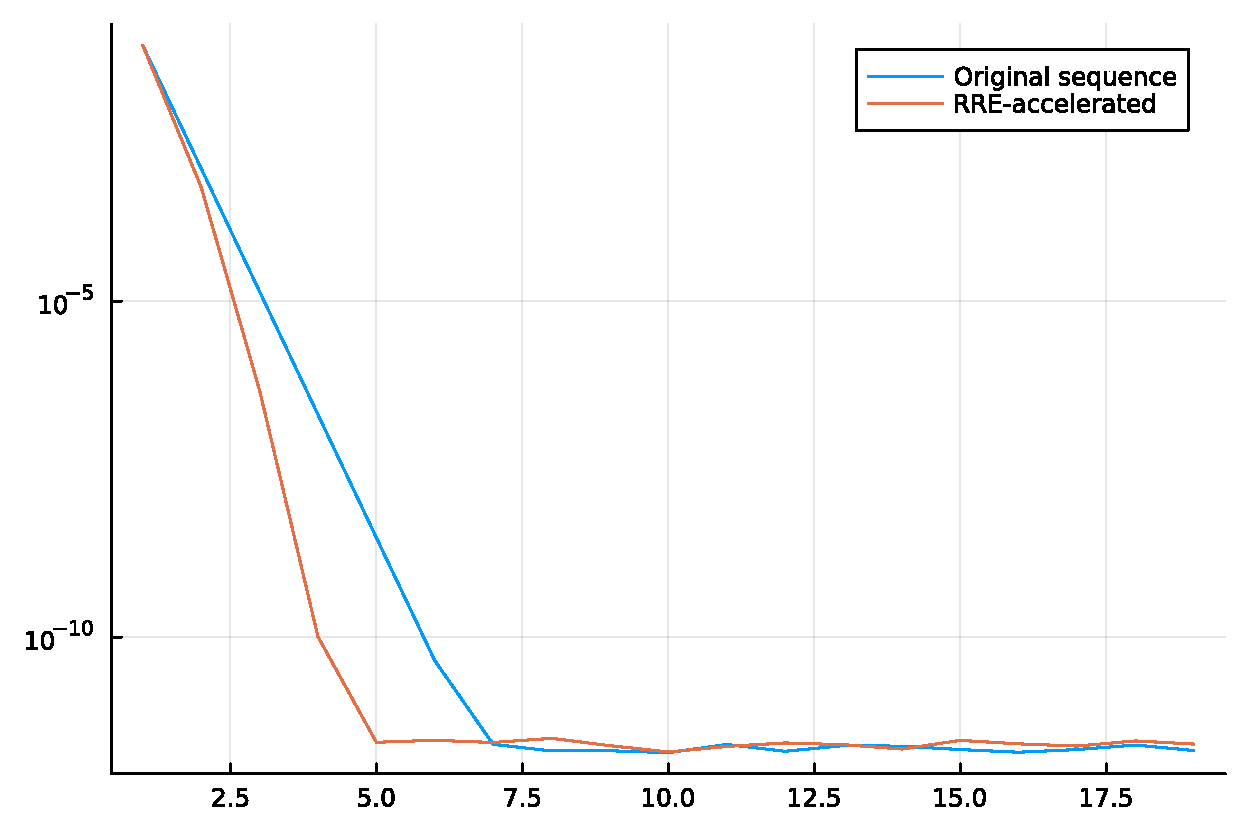
\includegraphics[width=0.8\textwidth]{fig/2023-04-14-rre.pdf}
\end{center}
\caption{Convergence of reduced-rank extrapolated simple fixed-point.}
\label{fig:rre-cvg}
\end{figure}

We plot convergence of reduced-rank extrapolation of the fixed point
iteration with $T_N$ as the Jacobian approximation in
Figure~\ref{fig:rre-cvg}.

\begin{minted}{julia}
function rre(X)
    m = size(X)[2]-1
    if m == 0
        return X[:,1]
    end
    F = qr(X[:,2:end]-X[:,1:end-1])
    y = F.R'\ones(m)
    γ = (F.R\y)/norm(y)^2
    return X[:,2:end]*γ
end
\end{minted}

When applied to a the iterates of a stationary iterative method for
solving \(Ax = b\), reduced rank extrapolation is formally the same as
the GMRES iteration. In numerical practice, though, the
orthogonalization that takes place when forming the Krylov subspace
bases in GMRES provides much better numerical stability than we would
get from RRE. Whether we apply the method to linear or nonlinear
problems, the matrices \(F_k\) in RRE are often rather ill-conditioned,
and the coefficient vectors \(\gamma\) have large positive and negative
entries, so that forming \(\sum_i \gamma_i x_{k+i}\) may lead to
significant cancellation. For this reason, one may want to choose modest
values of \(m\) in practice.

\subsection{Questions}

Explain why the QR-based algorithm given above to minimize
\(\|F_k \gamma\|^2\) subject to \(e^T \gamma = 1\) satisfies the
stationary conditions.

\section{Anderson acceleration}

Anderson acceleration is an old method, common in computational
chemistry, that has recently become popular for more varied problems
thanks to the work of Tim Kelley, Homer Walker, and various others. In
many ways, it is similar to reduced rank extrapolation applied to a
sequence of iterates from a fixed point iteration. If we wish to find
\(x_*\) such that \[f(x_*) = g(x_*)-x_* = 0\] then reduced rank
extrapolation -- without any linear algebra trickery -- at step \(k\)
looks like \begin{align*}
  m_k &= \min(m,k) \\
  F_k &= \begin{bmatrix} f(x_{k-m_k}) & \ldots & f(x_k) \end{bmatrix} \\
  \gamma^{(k)} &= \operatorname{argmin} \|F_k \gamma\|_2 \mbox{ s.t. } \sum_{i=0}^{m_k} = 1 \\
  s_{k+1} &= \sum_{i=0}^{m_k} \gamma_i^{(k)} g(x_{k-m_k+i})
\end{align*} In this application of reduced rank extrapolation, the
output sequence \(s_k\) and the input sequence \(x_k\) (defined by the
iteration \(x_{k+1} = g(x_k)\)) are distinct entities. By contrast, in
Anderson acceleration we have just one sequence: \begin{align*}
  m_k &= \min(m,k) \\
  F_k &= \begin{bmatrix} f(x_{k-m_k}) & \ldots & f(x_k) \end{bmatrix} \\
  \gamma^{(k)} &= \operatorname{argmin} \|F_k \gamma\|_2 \mbox{ s.t. } \sum_{i=0}^{m_k} = 1 \\
  x_{k+1} &= \sum_{i=0}^{m_k} \gamma_i^{(k)} g(x_{k-m_k+i})
\end{align*}

The only difference in the pseudocode is that the last step generates a
new \(x_{k+1}\) (which feeds into the next iteration), rather than
generating a separate output sequence \(s_{k+1}\) and computing the next
input iterate by a fixed point step. Thus, the difference between
Anderson acceleration and reduced rank extrapolation is morally the same
as the difference between Gauss-Seidel and Jacobi iteration: in the
former case, we try to work with the most recent guesses available.

Unsurprisingly, Anderson acceleration (like RRE) is equivalent to GMRES
when applied to linear fixed point iterations. Anderson acceleration can
also be seen as a multi-secant generalization of Broyden's iteration.
For a good overview of the literature and of different ways of thinking
about the method (as well as a variety of interesting applications), I
recommend ``\href{https://doi.org/10.1137/10078356X}{Anderson
Acceleration for Fixed-Point Iterations}'' by Walker and Ni (SIAM J.
Numer. Anal., Vol. 49, No.~4, pp.~1715--1735).

\begin{minted}{julia}
function anderson_step(X, gX)
    m = size(gX)[2]
    F = qr(gX-X)
    y = F.R'\ones(m)
    γ = (F.R\y)/norm(y)^2
    return gX*γ
end
\end{minted}

\begin{figure}
\begin{center}
  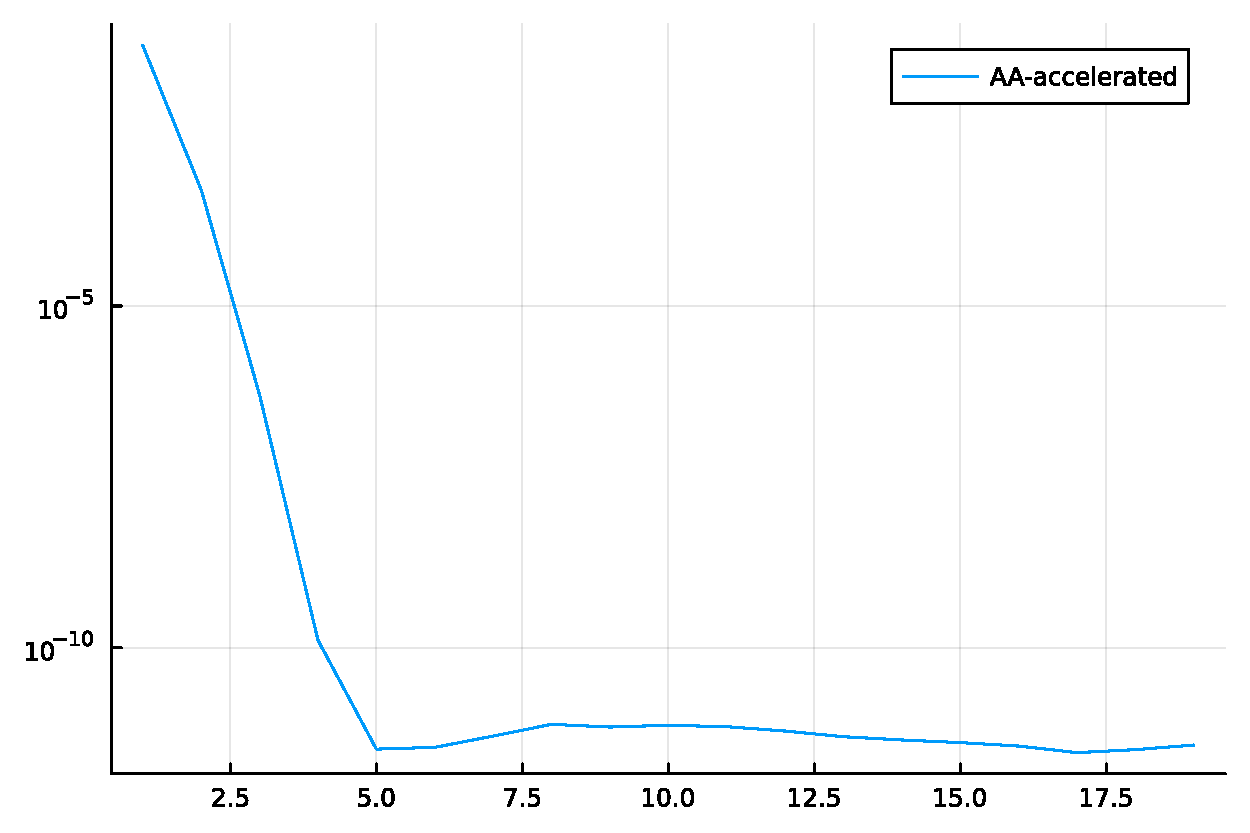
\includegraphics[width=0.8\textwidth]{fig/2023-04-14-aa.pdf}
\end{center}
\caption{Convergence of Anderson acceleration of a simple fixed-point.}
\label{fig:aa-cvg}
\end{figure}

We plot convergence of Anderson acceleration of the fixed point iteration
with $T_N$ as the Jacobian approximation in Figure~\ref{fig:aa-cvg}.


\end{document}
